% Simple circuit schematics symbols
% Author: Shengshan Cui
\documentclass{article}
\usepackage{tikz}
\usepackage{subfig}
\usepackage{verbatim}

\begin{comment}
:Title: Simple circuit schematics symbols
:Tags: Block diagrams, Paths

An example of how to create simple schematic symbols using paths and macros. The example also shows
how the symbols can be combined with the signalflow_ library by Karlheinz Ochs. For a general circuit 
library this should be done by creating `custom node shapes`_. However, that would require a lot more
work. 


| Author: `Shengshan Cui`_

.. _Shengshan Cui: http://web.njit.edu/~sc229/
.. _signalflow: http://www.fauskes.net/pgftikzexamples/signal-flow-building-blocks/
.. _custom node shapes: http://www.fauskes.net/pgftikzexamples/rectangle-node-with-diagonal-fill/

\end{comment}

\usepackage{signalflowdiagram}

% Define two simple circuit schematics symbols
\def\antenna{%
    -- +(0mm,4.0mm) -- +(2.625mm,7.5mm) -- +(-2.625mm,7.5mm) -- +(0mm,4.0mm)
}

\def\ground{%
    -- +(0mm,-4.0mm) {
        [yshift=-4mm]
        +(-2mm,0mm) -- +(2mm,0mm)
                +(-1mm,-1mm) -- +(1mm,-1mm)
                +(-0.3mm,-2mm) -- +(0.3mm,-2mm)
        }
}

\begin{document}

\begin{figure}
    \centering
    \subfloat[Stand alone symbols]{
        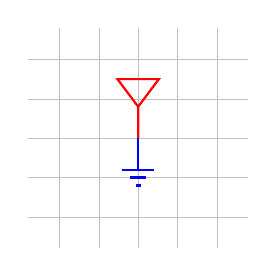
\begin{tikzpicture}
            \draw[step=.5cm,black!25,very thin] (-1.4,-1.4) grid (1.4,1.4);
            \draw[color=red,thick] (0,0) \antenna;
            \draw[color=blue,thick] (0,0) \ground;
        \end{tikzpicture}
    }\qquad
    \subfloat[Combining symbols with the signalflow library]{
        \begin{tikzpicture}
            \node[input]  (in)                   {$x(t)$};
            \node[delay]  (del) [right from=in]  {$T$};
            \node[coordinate] (out) [right from=del] {};
            % signal paths
            \path[r>] (in)  -- (del);
            \path[r] (del) -- (out) \antenna \ground;
        \end{tikzpicture}
    }
\end{figure}

\end{document}